\section{Referencia de la Clase Busqueda\-Proveedor}
\label{classBusquedaProveedor}\index{BusquedaProveedor@{BusquedaProveedor}}
Permite buscar y seleccionar un proveedor.  


{\tt \#include $<$busquedaproveedor.h$>$}

Diagrama de colaboraci\'{o}n para Busqueda\-Proveedor:\begin{figure}[H]
\begin{center}
\leavevmode
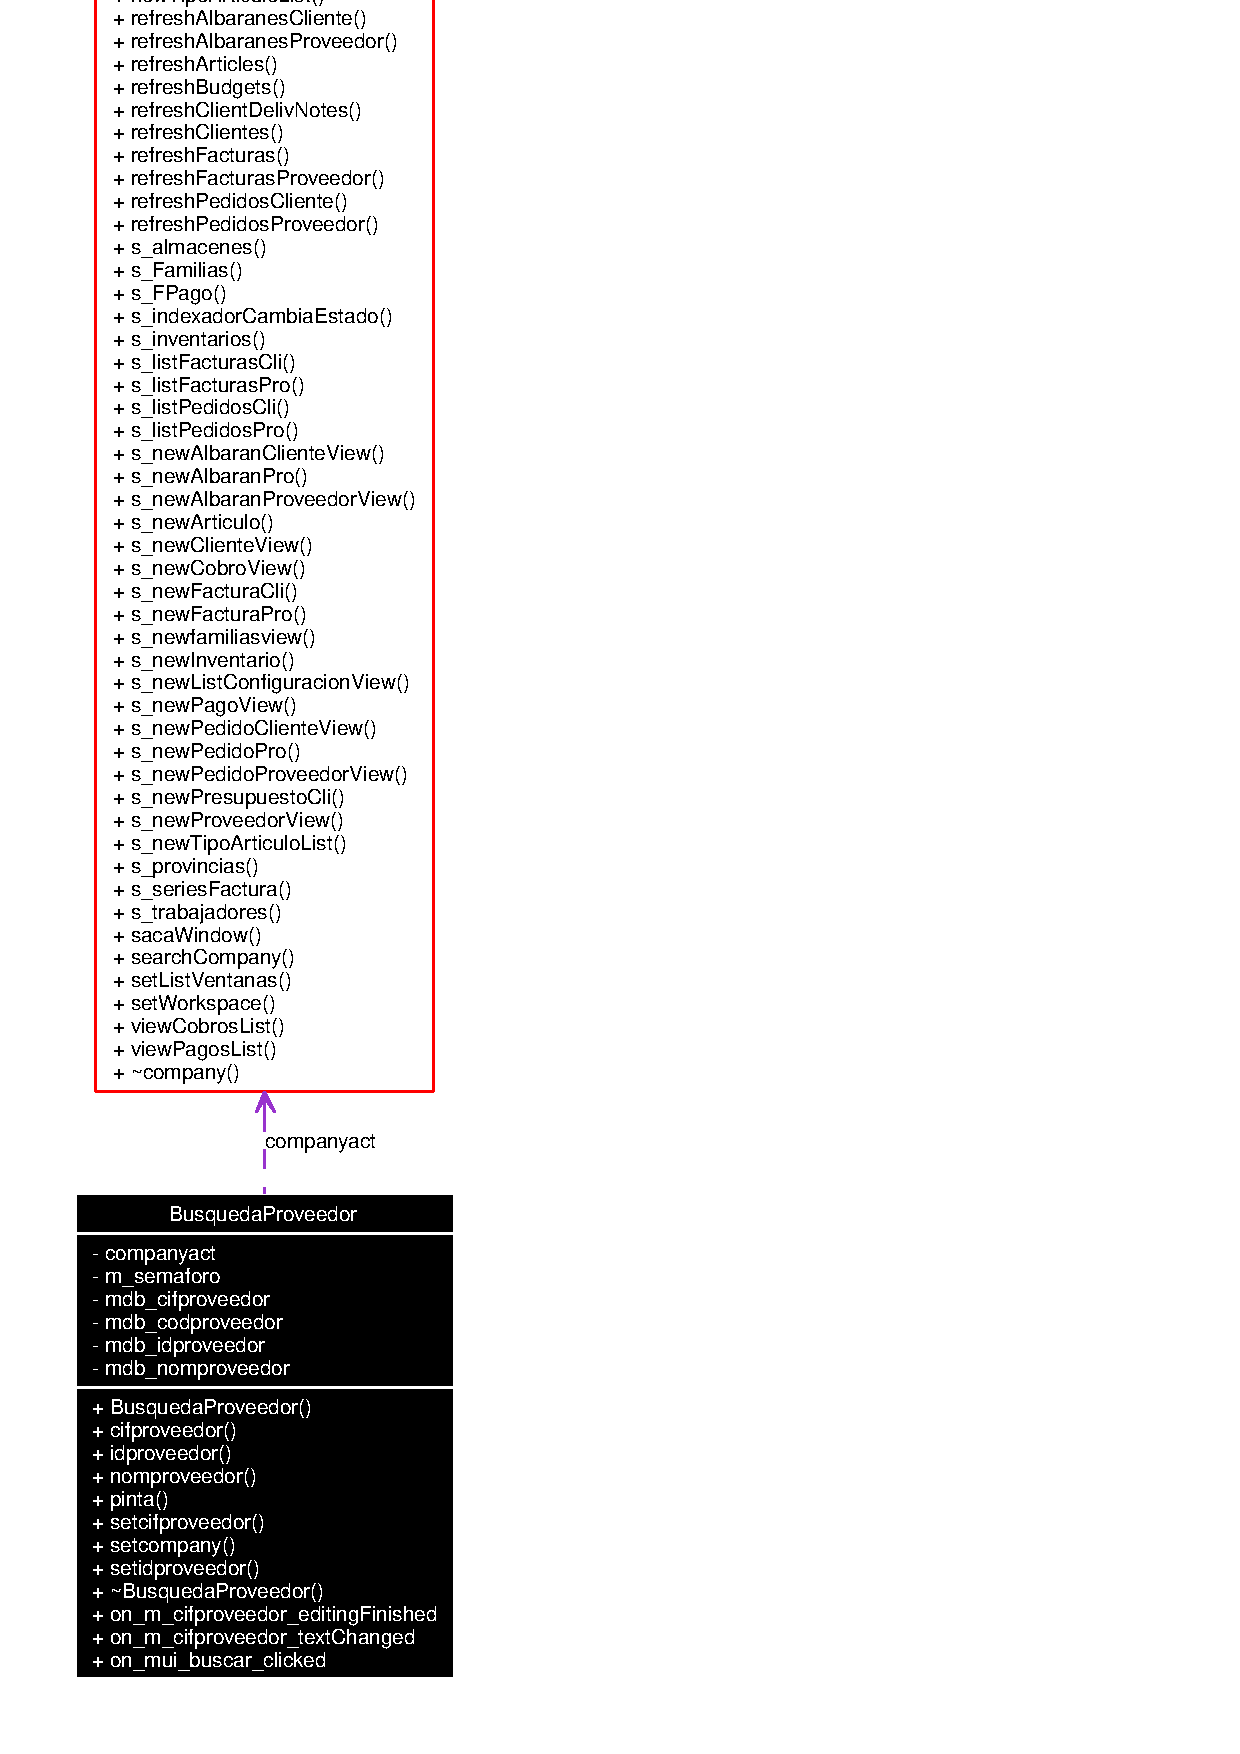
\includegraphics[width=109pt]{classBusquedaProveedor__coll__graph}
\end{center}
\end{figure}
\subsection*{Slots p\'{u}blicos}
\begin{CompactItemize}
\item 
virtual void {\bf on\_\-m\_\-cifproveedor\_\-editing\-Finished} ()\label{classBusquedaProveedor_i0}

\item 
virtual void {\bf on\_\-m\_\-cifproveedor\_\-text\-Changed} (const QString \&)\label{classBusquedaProveedor_i1}

\item 
virtual void {\bf on\_\-mui\_\-buscar\_\-clicked} ()
\begin{CompactList}\small\item\em Busqueda de proveedor. \item\end{CompactList}\end{CompactItemize}
\subsection*{Se\~{n}ales}
\begin{CompactItemize}
\item 
void {\bf value\-Changed} (QString)\label{classBusquedaProveedor_l0}

\end{CompactItemize}
\subsection*{M\'{e}todos p\'{u}blicos}
\begin{CompactItemize}
\item 
{\bf Busqueda\-Proveedor} (QWidget $\ast$parent=0)\label{classBusquedaProveedor_a0}

\item 
virtual QString {\bf cifproveedor} ()\label{classBusquedaProveedor_a1}

\item 
virtual QString {\bf idproveedor} ()\label{classBusquedaProveedor_a2}

\item 
virtual QString {\bf nomproveedor} ()\label{classBusquedaProveedor_a3}

\item 
void {\bf pinta} ()\label{classBusquedaProveedor_a4}

\item 
virtual void {\bf setcifproveedor} (QString val)\label{classBusquedaProveedor_a5}

\item 
void {\bf setcompany} ({\bf company} $\ast$comp)\label{classBusquedaProveedor_a6}

\item 
virtual void {\bf setidproveedor} (QString val)\label{classBusquedaProveedor_a7}

\end{CompactItemize}


\subsection{Descripci\'{o}n detallada}
Permite buscar y seleccionar un proveedor. 

Muestra la parte del formulario que permite buscar y seleccionar un proveedor. 



\subsection{Documentaci\'{o}n de las funciones miembro}
\index{BusquedaProveedor@{Busqueda\-Proveedor}!on_mui_buscar_clicked@{on\_\-mui\_\-buscar\_\-clicked}}
\index{on_mui_buscar_clicked@{on\_\-mui\_\-buscar\_\-clicked}!BusquedaProveedor@{Busqueda\-Proveedor}}
\subsubsection{\setlength{\rightskip}{0pt plus 5cm}void Busqueda\-Proveedor::on\_\-mui\_\-buscar\_\-clicked ()\hspace{0.3cm}{\tt  [virtual, slot]}}\label{classBusquedaProveedor_i2}


Busqueda de proveedor. 

Esto es convertir un QWidget en un sistema modal de dialogo. 

La documentaci\'{o}n para esta clase fu\'{e} generada a partir de los siguientes archivos:\begin{CompactItemize}
\item 
busquedaproveedor.h\item 
busquedaproveedor.cpp\end{CompactItemize}
